\chapter{Mutations et diversification des génomes}\label{ch:b2:genome-diversification}

Étalez un milliard de bactéries sur une boîte contenant un antibiotique~:
le lendemain matin, une poignée de colonies ont poussé. Le médicament
a-t-il appris à ces cellules à lui résister, ou étaient-elles déjà
résistantes avant de le rencontrer~? La question paraît philosophique~;
elle fut tranchée en 1943 par une expérience d'une grande élégance~: les
cellules résistantes étaient là auparavant, produites par des \omterm{def:b2:genome-diversification:mutation}{mutations}
survenues au hasard, sans égard à leur utilité. Ce chapitre traite des
sources de cette variation --- les erreurs de copie, les accidents
chimiques, les gènes sauteurs, les gènes échangés entre cellules, les
duplications de gènes et de génomes entiers --- et de leur vitesse. La
sélection, qui trie la variation, fait l'objet du
\cref{ch:b2:population-genetics}~; il s'agit ici de savoir d'où vient
la matière première.

\section{Les mutations}

\begin{definition}[La mutation et ses types]\label{def:b2:genome-diversification:mutation}
\index{mutation}\index{mutation ponctuelle}\index{decalage du cadre de lecture@décalage du cadre de lecture}\index{remaniement chromosomique}
Une \emph{mutation} est une modification héréditaire de la séquence du
génome. Les \emph{mutations ponctuelles} changent une ou quelques
bases~: une \emph{substitution} remplace une base par une autre (une
\emph{transition} échange une purine contre une purine ou une
pyrimidine contre une pyrimidine, A$\leftrightarrow$G ou C$\leftrightarrow$T~; une
\emph{transversion} échange les classes)~; une \emph{insertion} ou une
\emph{délétion} ajoute ou retire des bases. Dans une séquence codante,
une substitution est \emph{silencieuse} si le nouveau codon code le
même acide aminé, \emph{faux-sens} s'il en code un autre, \emph{non-sens}
s'il crée un codon stop~; une insertion ou une délétion dont la taille
n'est pas un multiple de trois décale le cadre de lecture
(\emph{décalage du cadre de lecture}) et brouille tous les codons en
aval. Les \emph{remaniements chromosomiques} déplacent de grands
segments~: délétion, duplication, inversion, translocation entre
chromosomes. Les \emph{mutations génomiques} changent le nombre de
chromosomes~: \emph{aneuploïdie} (un chromosome en trop ou en moins,
comme dans la trisomie 21) et \emph{\omterm{def:b2:genome-diversification:polyploidy}{polyploïdie}} (des jeux entiers
supplémentaires). Une mutation dans une cellule somatique n'est
transmise qu'aux descendantes de cette cellule~; une mutation dans la
lignée germinale est transmise aux descendants de l'organisme, et seules
ces dernières comptent pour l'évolution.
\end{definition}

\begin{omfigure}
\begin{tikzpicture}[every node/.style={font=\small\ttfamily}]
  \node[anchor=west] at (0,2.4) {ATG GAA TTC CTG AAG TGG TAA};
  \node[anchor=west, font=\scriptsize\rmfamily] at (5.6,2.4) {Met Glu Phe Leu Lys Trp stop --- type sauvage};
  \node[anchor=west] at (0,1.7) {ATG GA\textcolor{omThm}{G} TTC CTG AAG TGG TAA};
  \node[anchor=west, font=\scriptsize\rmfamily] at (5.6,1.7) {Met Glu Phe Leu Lys Trp stop --- silencieuse};
  \node[anchor=west] at (0,1.0) {ATG G\textcolor{omThm}{T}A TTC CTG AAG TGG TAA};
  \node[anchor=west, font=\scriptsize\rmfamily] at (5.6,1.0) {Met \textcolor{omThm}{Val} Phe Leu Lys Trp stop --- faux-sens};
  \node[anchor=west] at (0,0.3) {ATG \textcolor{omThm}{T}AA TTC CTG AAG TGG TAA};
  \node[anchor=west, font=\scriptsize\rmfamily] at (5.6,0.3) {Met \textcolor{omThm}{stop} --- non-sens};
  \node[anchor=west] at (0,-0.4) {ATG GA\textcolor{omThm}{C}A TTC CTG AAG TGG TAA};
  \node[anchor=west, font=\scriptsize\rmfamily] at (5.6,-0.4) {Met \textcolor{omThm}{Asp Ile Pro Glu Val} \dots{} --- décalage du cadre};
\end{tikzpicture}

{\small \omterm{def:b2:genome-diversification:mutation}{Mutations ponctuelles} dans une courte séquence codante (le
changement en rouge). Une substitution silencieuse conserve la
protéine~; une \omterm{def:b2:genome-diversification:mutation}{mutation} faux-sens change un résidu~; une \omterm{def:b2:genome-diversification:mutation}{mutation}
non-sens la tronque~; une seule base insérée décale le cadre et réécrit
tout ce qui suit.}
\end{omfigure}

\begin{proposition}[D'où viennent les mutations]\label{prop:b2:genome-diversification:sources}
\index{agent mutagene@agent mutagène}\index{desamination@désamination}\index{depurination@dépurination}
Trois sources. Les \emph{erreurs de réplication}~: l'ADN polymérase
place une base erronée environ une fois sur $10^{5}$~; son activité
exonucléase de relecture en élimine la plupart, n'en laissant qu'une
sur $10^{7}$~; la réparation des mésappariements, qui suit la fourche
de réplication et corrige le brin néosynthétisé d'après l'ancien, amène
le taux d'erreur final à environ $10^{-9}$ à $10^{-10}$ par base et par
réplication. La \emph{chimie spontanée}~: chaque jour, dans chaque
cellule humaine, quelque \num{10000} purines se détachent de leur sucre
(\emph{dépurination}) et une centaine de cytosines perdent un
groupement amine (\emph{désamination}, qui change C en U, lequel
s'apparie avec A)~; les deux lésions sont réparées, mais pas toujours.
Les \emph{\omterm{prop:b2:genome-diversification:sources}{agents mutagènes}}~: les ultraviolets soudent des thymines
adjacentes en dimères~; les rayonnements ionisants cassent les brins~;
les agents alkylants et l'acide nitreux modifient les bases~; les
colorants intercalants se glissent entre les paires de bases et
provoquent des décalages du cadre~; les radicaux oxygénés issus de la
respiration oxydent la guanine. Le taux par base est minuscule~;
multiplié par la taille d'un génome et par le nombre de cellules, il
ne l'est plus.
\end{proposition}

\begin{theorem}[Mutations par génome et par population]\label{thm:b2:genome-diversification:rate}
\index{taux de mutation}
Si le \omterm{thm:b2:genome-diversification:rate}{taux de mutation} est $u$ par paire de bases et par réplication et
que le génome compte $G$ paires de bases, chaque réplication produit en
moyenne $U = uG$ \omterm{def:b2:genome-diversification:mutation}{mutations} nouvelles, et une population de $N$ cellules
en produit $UN$ par génération. Pour \emph{E.~coli}
($u \approx \qty{5e-10}{}$, $G =
\qty{4.6e6}{}$)~: $U \approx 0.002$, si bien qu'une cellule sur cinq
cents porte une \omterm{def:b2:genome-diversification:mutation}{mutation} nouvelle --- mais une culture de $10^{9}$
cellules en produit deux millions par génération, et chacun des
$3G \approx 1.4\times
10^{7}$ changements possibles d'une seule base y apparaît quelque part
en quelques générations. Pour l'être humain ($u \approx \qty{1.2e-8}{}$
par génération, $G = \qty{3.2e9}{}$ par jeu haploïde, deux jeux)~:
chaque enfant porte environ \num{75} \omterm{def:b2:genome-diversification:mutation}{mutations} nouvelles, dont une ou
deux dans une séquence codante.
\end{theorem}
\begin{proof}
Chaque base est copiée indépendamment avec une probabilité d'erreur $u$~;
le nombre d'erreurs par copie du génome est donc la somme de $G$
événements rares indépendants, de moyenne $uG$ (et approximativement
distribuée selon une loi de Poisson). $N$ cellules font $N$ copies. Le
chiffre humain multiplie $u$ par $2G$ pour le génome diploïde~; le taux
est exprimé par génération et non par réplication, car les cellules
germinales subissent de nombreuses réplications entre une fécondation et
la suivante.
\end{proof}

\begin{theorem}[Les mutants dans une culture en croissance]\label{thm:b2:genome-diversification:luria}
\index{experience de Luria--Delbruck@expérience de Luria--Delbrück}\index{test de fluctuation}
Une culture qui passe de $N_0$ à $N$ cellules, dans laquelle une \omterm{def:b2:genome-diversification:mutation}{mutation}
donnée survient avec une probabilité $m$ à chaque division cellulaire,
contient à la fin un nombre moyen d'\emph{événements} mutationnels
$m(N - N_0)$, et un nombre moyen de \emph{cellules} mutantes
\[
\langle M\rangle = m\,N\,\ln\frac{N}{N_0},
\]
supérieur au nombre d'événements, car une \omterm{def:b2:genome-diversification:mutation}{mutation} précoce fonde un
clone. Le nombre de cellules mutantes varie énormément d'une culture à
l'autre (de rares événements précoces donnent des «~jackpots~»), alors
que si les \omterm{def:b2:genome-diversification:mutation}{mutations} étaient induites à l'étalement, il suivrait une loi
de Poisson de variance égale à sa moyenne. La proportion de cultures
sans aucun mutant vaut $p_0 = e^{-m(N - N_0)}$, ce qui donne
directement $m$.
\end{theorem}
\begin{proof}
La croissance de $n$ à $n + \mathrm{d}n$ cellules demande $\mathrm{d}n$
divisions, autant d'occasions de \omterm{def:b2:genome-diversification:mutation}{mutation}, si bien que $m\,\mathrm{d}n$
événements surviennent dans cet intervalle~; en sommant, $m(N - N_0)$
événements au total. Une \omterm{def:b2:genome-diversification:mutation}{mutation} survenue lorsque la culture compte $n$
cellules fonde un clone qui croît au même rythme que la culture et
compte $N/n$ cellules à la fin~; le nombre attendu de cellules mutantes
est donc
$\int_{N_0}^{N} m\,(N/n)\,\mathrm{d}n = mN\ln(N/N_0)$. Les événements
sont rares et indépendants~; leur nombre suit donc une loi de Poisson
de moyenne
$m(N - N_0)$, et la probabilité qu'il n'y en ait aucun vaut $e^{-m(N - N_0)}$.
\end{proof}
\begin{proof}[Faits expérimentaux]
Luria et Delbrück (1943) firent pousser vingt petites cultures
d'\emph{E.~coli} à partir de quelques cellules chacune et prélevèrent en
parallèle vingt échantillons d'une grande culture unique~; ils étalèrent
les quarante avec un bactériophage qui tue toute cellule sensible et
comptèrent les colonies résistantes. Les échantillons de la culture
unique donnèrent des nombres proches de leur moyenne, comme le prévoit
une loi de Poisson~; les cultures indépendantes donnèrent 0, 0, 1, 0, 3,
0, 107, 0, 5\dots{} --- une variance bien supérieure à la moyenne. Les
\omterm{def:b2:genome-diversification:mutation}{mutations} de résistance étaient survenues à des moments aléatoires
\emph{avant} que les cellules ne rencontrent le phage, les plus précoces
produisant des jackpots. Lederberg et Lederberg (1952) le confirmèrent
sans jamais exposer les cellules sélectionnées à l'agent~: en pressant un
tampon de velours sur une boîte pour en imprimer des copies, ils
trouvèrent des colonies résistantes aux mêmes positions sur toutes les
répliques, et les isolèrent à partir de la boîte mère non traitée.
\end{proof}

\begin{omfigure}
\begin{tikzpicture}[every node/.style={font=\scriptsize}, level distance=0.55cm, sibling distance=0.5cm, edge from parent/.style={draw, gray}]
  \begin{scope}
    \node[circle, fill=omDef!40, inner sep=1.5pt] (r) at (0,0) {}
      child { node[circle, fill=omDef!40, inner sep=1.5pt] {}
        child { node[circle, fill=omDef!40, inner sep=1.5pt] {} child { node[circle, fill=omDef!40, inner sep=1.5pt] {} } child { node[circle, fill=omDef!40, inner sep=1.5pt] {} } }
        child { node[circle, fill=omDef!40, inner sep=1.5pt] {} child { node[circle, fill=omDef!40, inner sep=1.5pt] {} } child { node[circle, fill=omThm, inner sep=1.5pt] {} } } }
      child { node[circle, fill=omDef!40, inner sep=1.5pt] {}
        child { node[circle, fill=omDef!40, inner sep=1.5pt] {} child { node[circle, fill=omDef!40, inner sep=1.5pt] {} } child { node[circle, fill=omDef!40, inner sep=1.5pt] {} } }
        child { node[circle, fill=omDef!40, inner sep=1.5pt] {} child { node[circle, fill=omDef!40, inner sep=1.5pt] {} } child { node[circle, fill=omDef!40, inner sep=1.5pt] {} } } };
    \node[align=center] at (0,-2.4) {mutation tardive~:\\une cellule mutante};
  \end{scope}
  \begin{scope}[xshift=5cm]
    \node[circle, fill=omDef!40, inner sep=1.5pt] at (0,0) {}
      child { node[circle, fill=omThm, inner sep=1.5pt] {}
        child { node[circle, fill=omThm, inner sep=1.5pt] {} child { node[circle, fill=omThm, inner sep=1.5pt] {} } child { node[circle, fill=omThm, inner sep=1.5pt] {} } }
        child { node[circle, fill=omThm, inner sep=1.5pt] {} child { node[circle, fill=omThm, inner sep=1.5pt] {} } child { node[circle, fill=omThm, inner sep=1.5pt] {} } } }
      child { node[circle, fill=omDef!40, inner sep=1.5pt] {}
        child { node[circle, fill=omDef!40, inner sep=1.5pt] {} child { node[circle, fill=omDef!40, inner sep=1.5pt] {} } child { node[circle, fill=omDef!40, inner sep=1.5pt] {} } }
        child { node[circle, fill=omDef!40, inner sep=1.5pt] {} child { node[circle, fill=omDef!40, inner sep=1.5pt] {} } child { node[circle, fill=omDef!40, inner sep=1.5pt] {} } } };
    \node[align=center] at (0,-2.4) {mutation précoce~:\\un jackpot de quatre};
  \end{scope}
  \begin{scope}[xshift=10cm]
    \node[circle, fill=omDef!40, inner sep=1.5pt] at (0,0) {}
      child { node[circle, fill=omDef!40, inner sep=1.5pt] {}
        child { node[circle, fill=omDef!40, inner sep=1.5pt] {} child { node[circle, fill=omDef!40, inner sep=1.5pt] {} } child { node[circle, fill=omThm, inner sep=1.5pt] {} } }
        child { node[circle, fill=omDef!40, inner sep=1.5pt] {} child { node[circle, fill=omDef!40, inner sep=1.5pt] {} } child { node[circle, fill=omDef!40, inner sep=1.5pt] {} } } }
      child { node[circle, fill=omDef!40, inner sep=1.5pt] {}
        child { node[circle, fill=omDef!40, inner sep=1.5pt] {} child { node[circle, fill=omThm, inner sep=1.5pt] {} } child { node[circle, fill=omDef!40, inner sep=1.5pt] {} } }
        child { node[circle, fill=omDef!40, inner sep=1.5pt] {} child { node[circle, fill=omDef!40, inner sep=1.5pt] {} } child { node[circle, fill=omDef!40, inner sep=1.5pt] {} } } };
    \node[align=center] at (0,-2.4) {si induite à l'étalement~:\\une dispersion de Poisson};
  \end{scope}
\end{tikzpicture}

{\small Le \omterm{thm:b2:genome-diversification:luria}{test de fluctuation}. Si les \omterm{def:b2:genome-diversification:mutation}{mutations} (en rouge) surviennent
au hasard pendant la croissance, le nombre de mutants dépend du
\emph{moment} où la \omterm{def:b2:genome-diversification:mutation}{mutation} s'est produite, et des cultures
indépendantes diffèrent énormément~; si l'agent sélectif les induisait
à l'étalement, toutes les cultures montreraient un petit nombre
comparable.}
\end{omfigure}

\begin{omfigure}
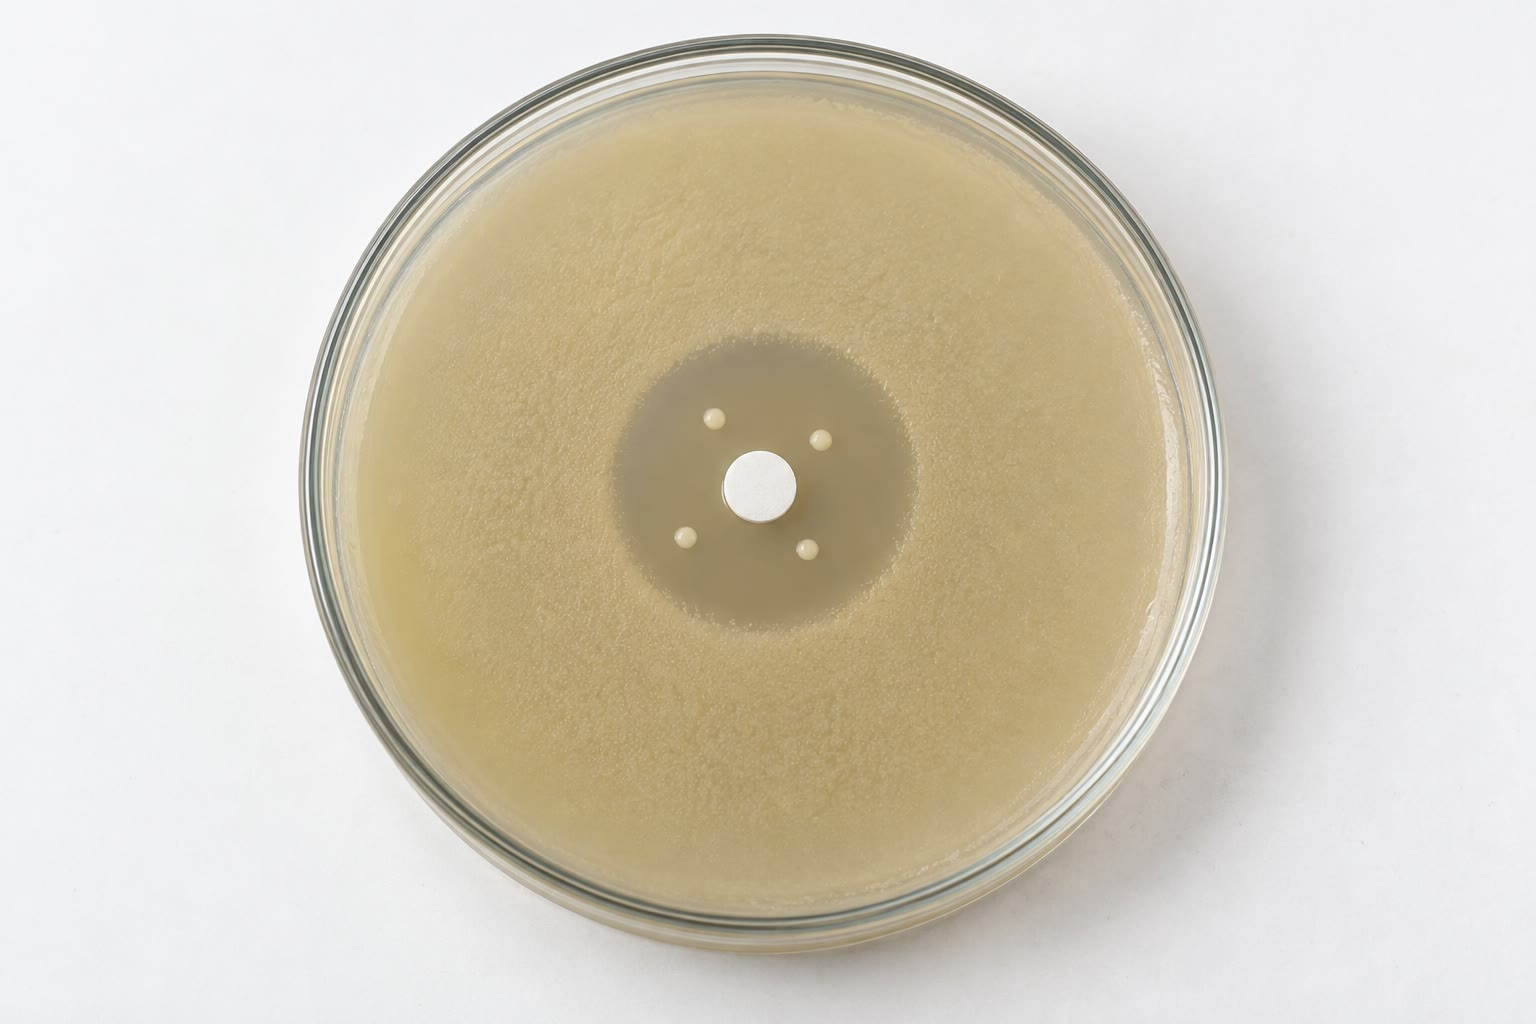
\includegraphics[width=0.5\linewidth]{images/book4/ai/b4-03-luria-plate.jpg}

{\small Un disque d'antibiotique sur un tapis bactérien~: la zone claire
est celle où le médicament diffusant du disque a tué les cellules
sensibles, et les colonies qui s'y trouvent sont issues de mutants
résistants présents avant la pose du disque.}
\end{omfigure}

\begin{proposition}[La réparation et ses limites]\label{prop:b2:genome-diversification:repair}
\index{reparation de l'ADN@réparation de l'ADN}
Une cellule corrige la plupart des lésions avant qu'elles ne deviennent
des \omterm{def:b2:genome-diversification:mutation}{mutations}. La \emph{réparation des mésappariements} retire la base
erronée du brin néosynthétisé. La \emph{réparation par excision de base}
découpe une seule base endommagée (un uracile, une guanine oxydée) et
comble la brèche~; c'est pourquoi l'ADN utilise la thymine plutôt que
l'uracile~: un uracile dans l'ADN ne peut être qu'une cytosine
désaminée, et il est reconnu comme étranger. La \emph{réparation par
excision de nucléotides} retire un segment d'une douzaine de bases
autour d'une lésion volumineuse comme un dimère de thymines~; les
personnes qui en sont dépourvues (xeroderma pigmentosum) développent des
cancers de la peau sous un ensoleillement ordinaire. La
\emph{réparation par recombinaison} reconstruit un chromosome cassé à
partir de sa copie sœur. Ce qui échappe à la réparation, ou est mal
réparé, est une \omterm{def:b2:genome-diversification:mutation}{mutation} --- et une cellule qui a perdu un système de
réparation (un \emph{mutateur}) mute cent fois plus vite, ce qui est un
avantage à court terme sous stress et un fardeau à long terme. Les
mécanismes de réparation sont traités en détail dans le volume de
troisième année.
\end{proposition}

\section{Les gènes qui se déplacent}

\begin{definition}[Les éléments transposables]\label{def:b2:genome-diversification:transposon}
\index{transposon}\index{retrotransposon@rétrotransposon}
Un \emph{élément transposable} est un segment d'ADN capable de se
déplacer vers une nouvelle position du génome. Les \emph{transposons à
ADN} codent une \emph{transposase} qui excise l'élément et le colle
ailleurs (ou l'y copie)~; les séquences d'insertion bactériennes sont
les plus simples (un gène de transposase entre deux répétitions
inversées), et les transposons composites portent des gènes
supplémentaires --- souvent des résistances aux antibiotiques --- entre
deux d'entre elles. Les \emph{rétrotransposons} se déplacent par une
voie de type copier-coller qui passe par un intermédiaire ARN, recopié
en ADN par une transcriptase inverse~; ils ne quittent jamais leur
ancien site et s'accumulent donc. Un élément qui s'insère dans un gène
l'interrompt~; inséré à proximité, il peut en modifier l'expression~;
deux copies sur un même chromosome offrent des sites de \omterm{prop:b2:genome-diversification:duplication}{crossing-over
inégal}. Les transposons et leurs vestiges forment la moitié du génome
humain et quatre-vingts pour cent du génome du maïs~; la plupart sont
aujourd'hui immobiles.
\end{definition}
\begin{proof}[Faits expérimentaux]
McClintock (années 1940--1950) étudia des grains de maïs dont le
pigment pourpre était perdu dans certaines cellules et restauré dans
d'autres, ce qui donnait des grains tachetés. Elle montra par des
croisements et par l'observation des chromosomes que cette instabilité
était due à un élément (\emph{Dissociation}) qui cassait le chromosome
là où il se trouvait et se déplaçait d'une position à l'autre sous le
contrôle d'un second élément (\emph{Activator}), et qu'un gène était
réduit au silence quand l'élément s'y trouvait et réactivé quand il en
partait. Les gènes, conclut-elle, pouvaient changer de position~;
l'idée ne fut acceptée que vingt ans plus tard, lorsqu'on découvrit les
séquences d'insertion bactériennes, et lui valut le prix Nobel en 1983.
\end{proof}

\begin{omfigure}
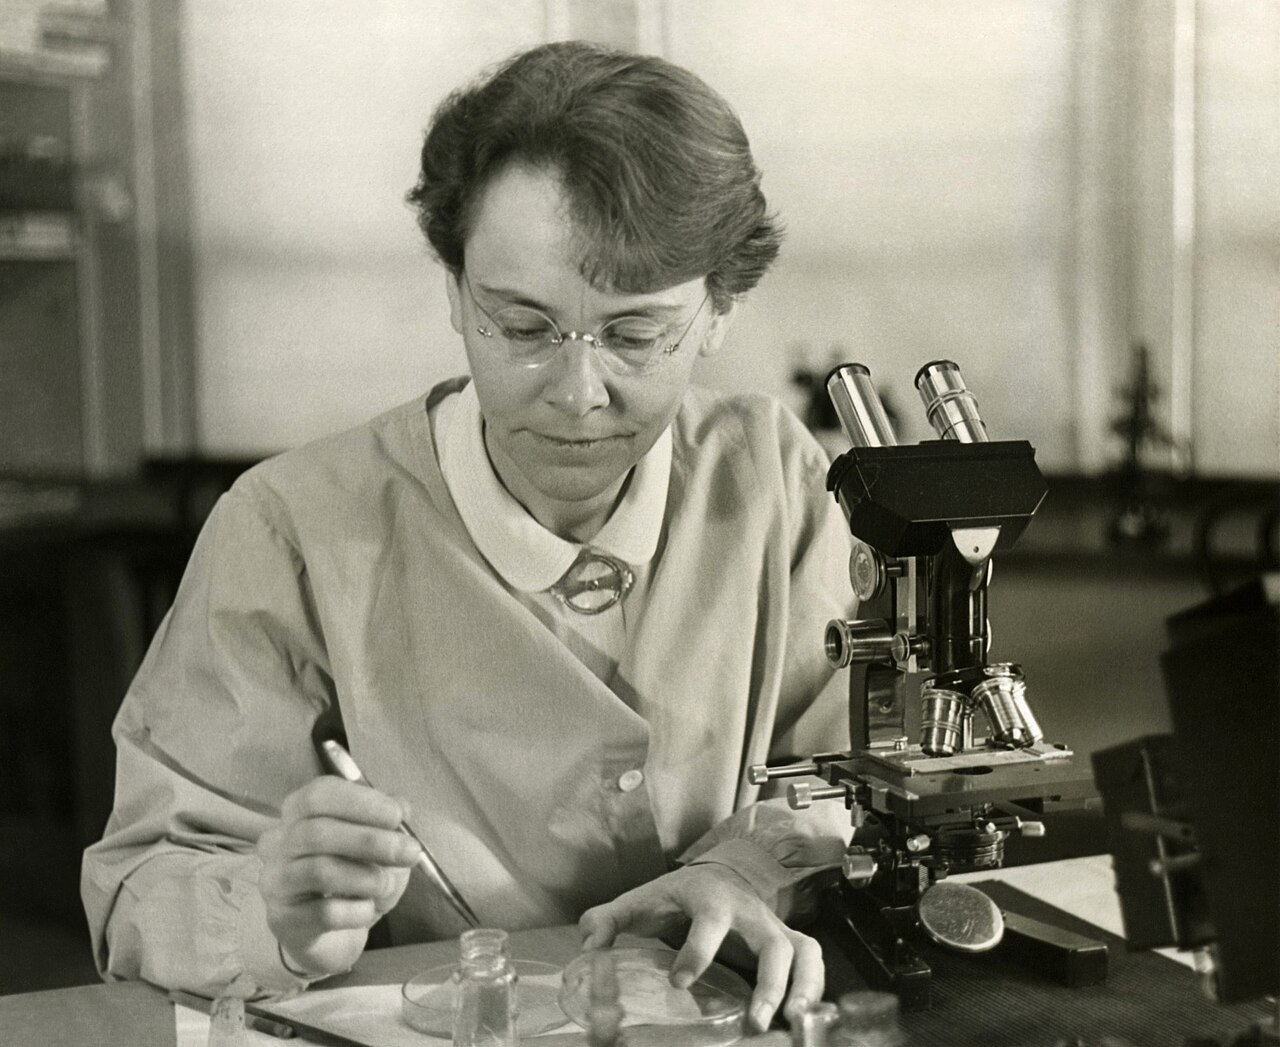
\includegraphics[width=0.4\linewidth]{images/book4/mcclintock.jpg}\hspace{0.04\linewidth}
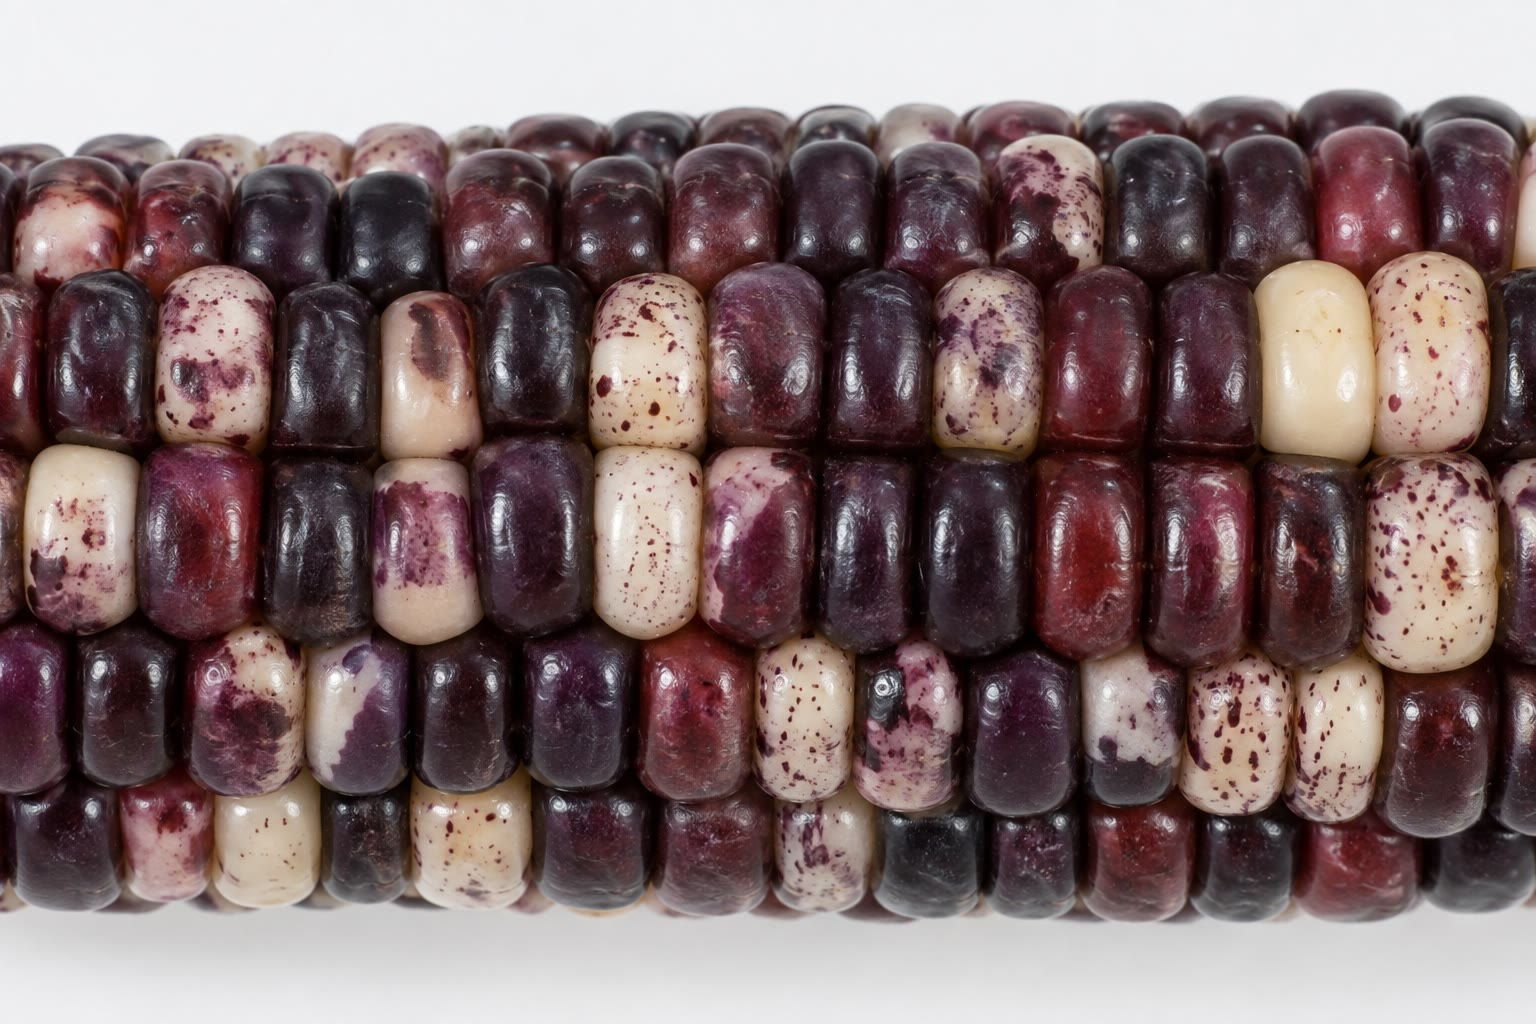
\includegraphics[width=0.5\linewidth]{images/book4/ai/b4-03-maize-kernels.jpg}

{\small Barbara McClintock, et les grains qui la conduisirent aux
éléments transposables~: un gène de pigment pourpre éteint par un
élément inséré, puis rallumé, cellule par cellule, lorsque l'élément
s'échappe, laissant des taches et des secteurs.}
\end{omfigure}

\begin{omfigure}
\begin{tikzpicture}[every node/.style={font=\scriptsize}]
  % cut and paste
  \begin{scope}
    \draw[very thick, gray] (0,1.2) -- (4.5,1.2);
    \fill[omThm!70] (0.8,1.05) rectangle (1.8,1.35); \node[white, font=\tiny] at (1.3,1.2) {Tn};
    \draw[very thick, gray] (0,0) -- (4.5,0);
    \fill[omThm!70] (2.8,-0.15) rectangle (3.8,0.15); \node[white, font=\tiny] at (3.3,0) {Tn};
    \draw[->, thick, omThm] (1.3,1.0) .. controls (1.3,0.5) and (3.3,0.7) .. (3.3,0.2);
    \draw[dashed, gray] (0.8,1.2) -- (1.8,1.2);
    \node[align=center] at (2.25,-0.6) {couper-coller (transposon à ADN)~:\\l'élément quitte son ancien site};
  \end{scope}
  % copy and paste
  \begin{scope}[xshift=7.5cm]
    \draw[very thick, gray] (0,1.2) -- (4.5,1.2);
    \fill[omProp!80] (0.8,1.05) rectangle (1.8,1.35); \node[white, font=\tiny] at (1.3,1.2) {RT};
    \draw[very thick, gray] (0,0) -- (4.5,0);
    \fill[omProp!80] (2.8,-0.15) rectangle (3.8,0.15); \node[white, font=\tiny] at (3.3,0) {RT};
    \draw[->, thick, omProp] (1.3,1.0) .. controls (1.3,0.5) and (3.3,0.7) .. (3.3,0.2);
    \node[omProp, anchor=west, align=left] at (3.6,0.75) {copie ARN,\\rétrotranscrite};
    \node[align=center] at (2.25,-0.6) {copier-coller (rétrotransposon)~:\\l'ancienne copie reste, le nombre croît};
  \end{scope}
\end{tikzpicture}

{\small Deux manières de se déplacer. Un \omterm{def:b2:genome-diversification:transposon}{transposon} à ADN est excisé
puis réinséré~; un \omterm{def:b2:genome-diversification:transposon}{rétrotransposon} est transcrit, recopié en ADN et
inséré ailleurs, si bien que ses copies s'accumulent.}
\end{omfigure}

\begin{definition}[Le transfert horizontal de gènes]\label{def:b2:genome-diversification:hgt}
\index{transfert horizontal de genes@transfert horizontal de gènes}\index{transformation}\index{conjugaison!bacterienne@bactérienne}\index{transduction}
Les \omterm{def:b2:unicellular-diversity:prokaryote}{procaryotes} acquièrent des gènes de cellules qui ne sont pas leurs
parents par trois voies. La \emph{transformation}~: une cellule absorbe
de l'ADN nu présent dans son milieu (libéré par des cellules mortes) et
l'intègre par recombinaison à son chromosome~; certaines espèces sont
naturellement compétentes, et c'est par cette voie que les pneumocoques
échangent leurs gènes de capsule. La \emph{conjugaison}~: un donneur
portant un \omterm{def:b2:unicellular-diversity:prokaryote}{plasmide} conjugatif (le facteur F
d'\emph{E.~coli}) construit un pilus, attire un receveur contre lui et
lui transmet un simple brin du \omterm{def:b2:unicellular-diversity:prokaryote}{plasmide} à travers un pore tout en le
répliquant selon le cercle roulant~; si le \omterm{def:b2:unicellular-diversity:prokaryote}{plasmide} s'est intégré au
chromosome (souche Hfr), des gènes chromosomiques sont transférés à sa
suite dans un ordre fixe, et le moment où chacun entre permet de
cartographier le chromosome. La \emph{transduction}~: un bactériophage
empaquette par erreur un fragment d'ADN de l'hôte et l'injecte dans la
cellule suivante qu'il infecte. Ensemble, ces voies font passer des
gènes de résistance d'une espèce à l'autre dans les hôpitaux en
quelques années, et ont déplacé des gènes métaboliques à travers tout
l'arbre bactérien au cours des temps géologiques, si bien que
l'ascendance d'un \omterm{def:b2:unicellular-diversity:prokaryote}{procaryote} est un réseau autant qu'un arbre
(\cref{ch:b2:phylogenetic-trees}).
\end{definition}
\begin{proof}[Faits expérimentaux]
Lederberg et Tatum (1946) mélangèrent deux souches d'\emph{E.~coli},
chacune incapable de fabriquer deux nutriments différents, et étalèrent
le mélange sur un milieu minimum sur lequel aucune ne pouvait pousser
seule~: des colonies apparurent, à raison d'environ une pour dix
millions de cellules, capables de fabriquer les quatre --- des
recombinants. Davis (1950) répéta l'expérience en séparant les souches
par un filtre qui laissait passer les molécules mais pas les cellules~:
aucun recombinant, le contact était donc nécessaire. Hayes montra
ensuite que le transfert était à sens unique, d'un donneur vers un
receveur, et Wollman et Jacob (1956) interrompirent les conjugaisons
dans un mixeur à intervalles réguliers et virent les gènes du donneur
entrer dans le receveur dans un ordre fixe, l'un après l'autre, en une
centaine de minutes environ.
\end{proof}

\begin{omfigure}
\begin{minipage}[b]{0.56\linewidth}\centering
\begin{tikzpicture}[every node/.style={font=\scriptsize}]
  % donor
  \draw[thick, fill=omDef!8] (0,0) ellipse (1.5 and 0.75);
  \draw[thick, omDef] (0.2,0) circle (0.45);
  \draw[thick, omThm] (-0.9,0.1) circle (0.22);
  \node[anchor=south] at (0,1.25) {donneur $F^+$};
  \draw[omThm] (-0.9,-0.12) -- (-1.1,-1.0) node[below] {plasmide F};
  \draw[omDef] (0.4,-0.4) -- (0.6,-1.0) node[below] {chromosome};
  % recipient
  \draw[thick, fill=omDef!8] (5,0) ellipse (1.5 and 0.75);
  \draw[thick, omDef] (5.2,0) circle (0.45);
  \node[anchor=south] at (5,1.25) {receveur $F^-$};
  % pilus
  \draw[very thick, omThm] (1.5,0) -- (3.5,0);
  \node[omThm, below] at (2.5,-0.05) {pilus};
  % single strand transferred
  \draw[->, thick, omThm, dashed] (-0.7,0.15) .. controls (1.0,0.7) and (3.0,0.7) .. (4.1,0.4);
  \node[omThm, anchor=south] at (2.5,0.7) {un brin copié selon le cercle roulant};
  \draw[thick, omThm, dashed] (4.1,0.2) circle (0.2);
\end{tikzpicture}
\end{minipage}\hfill
\begin{minipage}[b]{0.42\linewidth}\centering
\begin{tikzpicture}
\begin{axis}[
  width=\linewidth, height=4.6cm,
  axis x line=bottom, axis y line=left,
  xmin=0, xmax=40, ymin=0, ymax=1.1,
  xlabel={minutes avant le passage au mixeur}, ylabel={recombinants (relatif)},
  xlabel style={font=\scriptsize, at={(axis description cs:0.5,-0.18)}, anchor=north},
  ylabel style={font=\scriptsize},
  tick label style={font=\scriptsize}, xtick={0,10,20,30,40}, ytick={0,0.5,1},
  legend style={font=\scriptsize, at={(0.97,0.08)}, anchor=south east, draw=none},
  clip=false,
]
\addplot[very thick, omDef, domain=8:40, samples=40] {1-exp(-(x-8)/5)};
\addlegendentry{\emph{thr}, entre à \qty{8}{min}}
\addplot[very thick, omProp, domain=17:40, samples=40] {1-exp(-(x-17)/5)};
\addlegendentry{\emph{lac}, \qty{17}{min}}
\addplot[very thick, omThm, domain=25:40, samples=40] {1-exp(-(x-25)/5)};
\addlegendentry{\emph{gal}, \qty{25}{min}}
\end{axis}
\end{tikzpicture}
\end{minipage}

{\small À gauche~: la conjugaison --- le donneur transmet un brin de son
\omterm{def:b2:unicellular-diversity:prokaryote}{plasmide} F à travers la jonction du pilus tout en le copiant. À
droite~: l'expérience de conjugaison interrompue avec un donneur Hfr~:
chaque gène chromosomique commence à apparaître parmi les recombinants
à un moment caractéristique, ce qui cartographie le chromosome en
minutes.}
\end{omfigure}

\begin{omfigure}
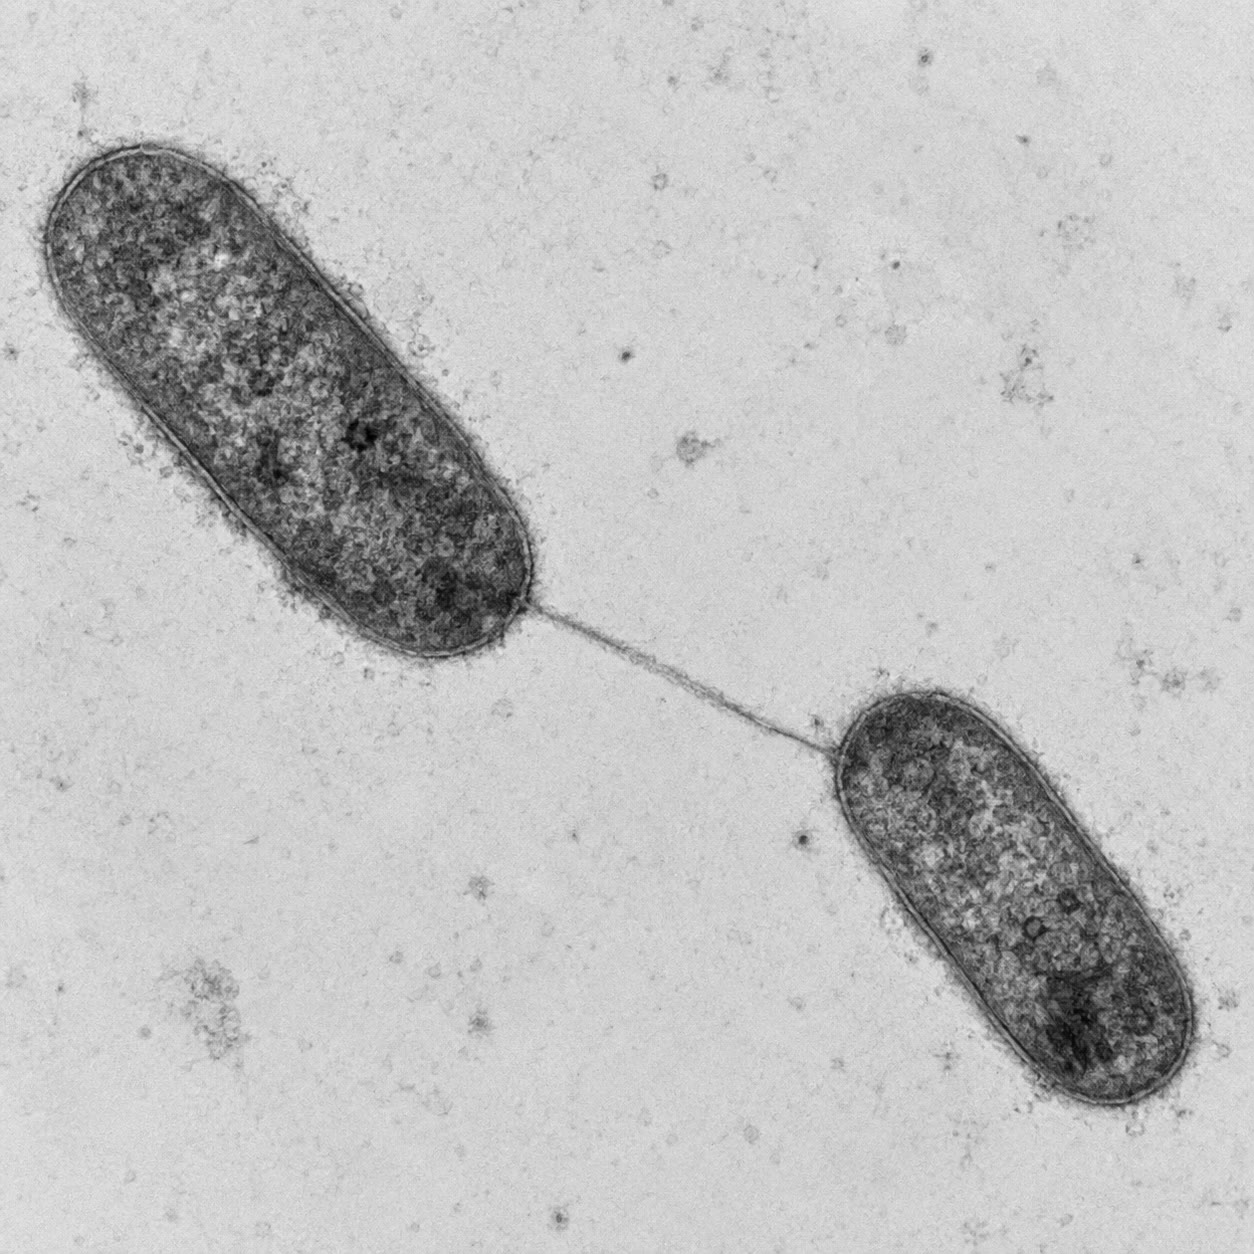
\includegraphics[width=0.42\linewidth]{images/book4/ai/b4-03-conjugation-tem.jpg}

{\small Deux bactéries reliées par un pilus conjugatif, observées en
microscopie électronique à transmission~: le pont par lequel passe le
\omterm{def:b2:unicellular-diversity:prokaryote}{plasmide}.}
\end{omfigure}

\begin{example}[La résistance en mouvement]\label{ex:b2:genome-diversification:resistance}
Un gène de résistance apparaît typiquement une seule fois, par \omterm{def:b2:genome-diversification:mutation}{mutation}
ou chez la bactérie du sol qui fabrique l'antibiotique, puis il
voyage~: d'un chromosome vers un \omterm{def:b2:genome-diversification:transposon}{transposon}, du \omterm{def:b2:genome-diversification:transposon}{transposon} vers un
\omterm{def:b2:unicellular-diversity:prokaryote}{plasmide} conjugatif, du \omterm{def:b2:unicellular-diversity:prokaryote}{plasmide} d'une espèce à l'autre par conjugaison
et d'une souche à l'autre par \omterm{def:b2:genome-diversification:hgt}{transduction}, puis de nouveau dans un
chromosome par \omterm{def:b2:genome-diversification:hgt}{transformation}. Des \omterm{def:b2:unicellular-diversity:prokaryote}{plasmides} portant cinq ou six
résistances à la fois (assemblées dans des \emph{intégrons}, qui
capturent des cassettes de gènes) furent découverts au Japon dans les
années 1950, quelques années après l'entrée en usage des médicaments~;
le gène de la carbapénémase NDM-1, observé pour la première fois en
2008, avait atteint tous les continents trois ans plus tard, porté par
un \omterm{def:b2:unicellular-diversity:prokaryote}{plasmide}. L'évolution de la résistance est surtout, non l'évolution
de gènes nouveaux, mais le déplacement de gènes anciens.
\end{example}

\section{La duplication~: gènes et génomes}

\begin{proposition}[Duplication génique et familles multigéniques]\label{prop:b2:genome-diversification:duplication}
\index{duplication genique@duplication génique}\index{famille multigenique@famille multigénique}\index{crossing-over inegal@crossing-over inégal}
Lorsque deux séquences semblables se suivent en tandem sur un
chromosome, les homologues peuvent s'apparier en décalé à la méiose et
effectuer un \omterm{prop:b2:genome-diversification:duplication}{crossing-over inégal}, si bien qu'un produit porte trois
copies et l'autre une seule. Un gène dupliqué est redondant~: une copie
peut conserver l'ancienne fonction tandis que l'autre accumule
librement les \omterm{def:b2:genome-diversification:mutation}{mutations} --- le plus souvent en dégénérant en
\emph{pseudogène}, parfois en acquérant une fonction nouvelle
(\emph{néofonctionnalisation}) ou une part de l'ancienne
(\emph{sous-fonctionnalisation}). Répété pendant des centaines de
millions d'années, ce processus construit des \emph{\omterm{prop:b2:genome-diversification:duplication}{familles
multigéniques}}~: les globines (un seul gène ancestral est devenu la
myoglobine, le groupe $\alpha$ et le groupe
$\beta$, dont les membres embryonnaires, fœtaux et adultes s'expriment
successivement), les récepteurs olfactifs (un millier de gènes chez la
souris), les gènes à homéoboîte, les cristallines du cristallin. La
plupart des gènes d'un génome appartiennent à une famille, et la
duplication est la principale source de gènes nouveaux.
\end{proposition}
\begin{proof}[Faits expérimentaux]
Le groupe de la $\beta$-globine humaine, sur le chromosome 11, compte
cinq gènes fonctionnels ($\varepsilon$, $^{G}\gamma$, $^{A}\gamma$,
$\delta$, $\beta$) et un pseudogène, dans l'ordre où ils s'activent au
cours du développement, tous avec la même structure exon--intron, et
des séquences d'autant plus semblables qu'ils ont divergé plus
récemment~; le groupe $\alpha$, sur le chromosome 16, a la même
architecture. Les délétions d'un ou plusieurs gènes $\alpha$, produites
par \omterm{prop:b2:genome-diversification:duplication}{crossing-over inégal} entre les copies presque identiques, sont
fréquentes et causent l'$\alpha$-thalassémie~; le produit réciproque,
un chromosome portant trois gènes $\alpha$, se rencontre dans les mêmes
populations.
\end{proof}

\begin{omfigure}
\begin{tikzpicture}[every node/.style={font=\scriptsize}]
  % unequal crossing over
  \begin{scope}
    \draw[very thick, gray] (0,1.2) -- (5,1.2);
    \fill[omDef!70] (1.0,1.05) rectangle (2.0,1.35); \fill[omDef!70] (2.4,1.05) rectangle (3.4,1.35);
    \draw[very thick, gray] (0,0) -- (5,0);
    \fill[omDef!70] (1.0,-0.15) rectangle (2.0,0.15); \fill[omDef!70] (2.4,-0.15) rectangle (3.4,0.15);
    \node[above] at (1.5,1.35) {A}; \node[above] at (2.9,1.35) {A$'$};
    \draw[very thick, omThm] (2.9,1.05) -- (1.5,0.15);
    \node[align=center] at (2.5,-0.6) {homologues mal appariés~:\\crossing-over inégal};
    \draw[->, thick, gray] (5.3,0.6) -- (6.1,0.6);
    % products
    \draw[very thick, gray] (6.5,1.2) -- (11.5,1.2);
    \fill[omDef!70] (7.5,1.05) rectangle (8.5,1.35); \fill[omDef!70] (8.9,1.05) rectangle (9.9,1.35); \fill[omDef!70] (10.3,1.05) rectangle (11.3,1.35);
    \node[above] at (9.4,1.35) {trois copies};
    \draw[very thick, gray] (6.5,0) -- (11.5,0);
    \fill[omDef!70] (7.5,-0.15) rectangle (8.5,0.15);
    \node[above] at (8.0,0.15) {une copie};
  \end{scope}
  % globin family tree
  \begin{scope}[yshift=-3.6cm]
    \draw[thick] (2,2.2) -- (2,1.7);
    \draw[thick] (0.5,1.7) -- (3.5,1.7);
    \draw[thick] (0.5,1.7) -- (0.5,0.4); \node[below] at (0.5,0.4) {myoglobine};
    \draw[thick] (3.5,1.7) -- (3.5,1.2);
    \draw[thick] (2.3,1.2) -- (4.7,1.2);
    \draw[thick] (2.3,1.2) -- (2.3,0.4); \node[below] at (2.3,0.4) {famille $\alpha$};
    \draw[thick] (4.7,1.2) -- (4.7,0.9);
    \draw[thick] (3.6,0.9) -- (5.8,0.9);
    \draw[thick] (3.6,0.9) -- (3.6,0.4); \node[below] at (3.6,0.4) {$\varepsilon,\gamma$};
    \draw[thick] (5.8,0.9) -- (5.8,0.7);
    \draw[thick] (5.2,0.7) -- (6.4,0.7);
    \draw[thick] (5.2,0.7) -- (5.2,0.4); \node[below] at (5.2,0.4) {$\delta$};
    \draw[thick] (6.4,0.7) -- (6.4,0.4); \node[below] at (6.4,0.4) {$\beta$};
    \node[anchor=west, align=left] at (7.2,1.7) {duplications d'un gène de globine ancestral~:\\avant les vertébrés (myoglobine/hémoglobine),\\il y a $\sim$450 millions d'années ($\alpha$/$\beta$),\\puis au sein du groupe $\beta$ (embryonnaire, fœtal, adulte)};
    \node[anchor=east, gray] at (1.9,2.1) {globine ancestrale};
  \end{scope}
\end{tikzpicture}

{\small En haut~: un \omterm{prop:b2:genome-diversification:duplication}{crossing-over inégal} entre copies en tandem mal
appariées produit un chromosome à trois copies et un chromosome à une
seule copie. En bas~: la famille des globines, construite par
duplications et divergences successives.}
\end{omfigure}

\begin{definition}[La polyploïdie]\label{def:b2:genome-diversification:polyploidy}
\index{polyploidie@polyploïdie}\index{allopolyploide@allopolyploïde}\index{autopolyploide@autopolyploïde}
Un \emph{polyploïde} porte plus de deux jeux complets de chromosomes.
Un \emph{autopolyploïde} possède plusieurs jeux issus d'une même espèce
(une méiose ratée donne un gamète diploïde~; deux gamètes de ce type
donnent un tétraploïde)~; un \emph{allopolyploïde} associe les jeux de
deux espèces après une hybridation. L'hybride diploïde AB, où aucun
chromosome n'a d'homologue, ne peut pas les apparier à la méiose et il
est stérile~; si son génome double pour donner AABB, chaque chromosome
retrouve un partenaire, la méiose fonctionne et la nouvelle plante est
fertile --- mais elle ne peut plus se croiser avec aucun des deux
parents (un descendant AAB est stérile). La polyploïdie crée ainsi une
espèce nouvelle en une seule étape, et environ un tiers des espèces de
plantes à fleurs sont apparues de cette façon~: le blé tendre est un
hexaploïde AABBDD issu de trois graminées, le fraisier cultivé un
octoploïde, le cotonnier et le tabac des allotétraploïdes, et la lignée
des vertébrés elle-même a doublé deux fois son génome près de son
origine. Les polyploïdes sont en général plus grands que leurs ancêtres
diploïdes (plus d'ADN, des cellules plus grosses) et très recherchés par
les sélectionneurs.
\end{definition}

\begin{omfigure}
\begin{tikzpicture}[every node/.style={font=\scriptsize}]
  \node[draw, rounded corners, fill=omDef!10, align=center] (a) at (0,0) {\emph{T.~urartu}\\AA, $2n = 14$};
  \node[draw, rounded corners, fill=omDef!10, align=center] (b) at (3.4,0) {\emph{Aegilops}\\BB, $2n = 14$};
  \node[draw, rounded corners, fill=omProp!15, align=center] (ab) at (1.7,-1.5) {hybride AB\\$n = 14$, stérile};
  \node[draw, rounded corners, fill=omExo!25, align=center] (aabb) at (1.7,-3.1) {blé amidonnier AABB\\$2n = 28$, fertile};
  \node[draw, rounded corners, fill=omDef!10, align=center] (d) at (6.4,-3.1) {\emph{Ae.~tauschii}\\DD, $2n = 14$};
  \node[draw, rounded corners, fill=omProp!15, align=center] (abd) at (4.0,-4.6) {hybride ABD\\$3n = 21$, stérile};
  \node[draw, rounded corners, fill=omExo!25, align=center] (abd2) at (4.0,-6.1) {blé tendre AABBDD\\$2n = 42$, fertile};
  \draw[->, thick] (a) -- (ab); \draw[->, thick] (b) -- (ab);
  \draw[->, thick] (ab) -- (aabb) node[midway, right] {doublement du génome};
  \draw[->, thick] (aabb) -- (abd); \draw[->, thick] (d) -- (abd);
  \draw[->, thick] (abd) -- (abd2) node[midway, right] {doublement du génome};
  \node[anchor=west, align=left, gray] at (7.8,-1.5) {chaque hybridation donne une plante\\stérile aux chromosomes non appariés~;\\chaque doublement rétablit l'appariement\\et la fertilité --- et crée une\\espèce qui ne peut plus se recroiser};
\end{tikzpicture}

{\small L'origine du blé tendre~: deux hybridations, chacune suivie d'un
doublement du génome, ont construit un hexaploïde à partir de trois
graminées diploïdes en une dizaine de milliers d'années.}
\end{omfigure}

\begin{omfigure}
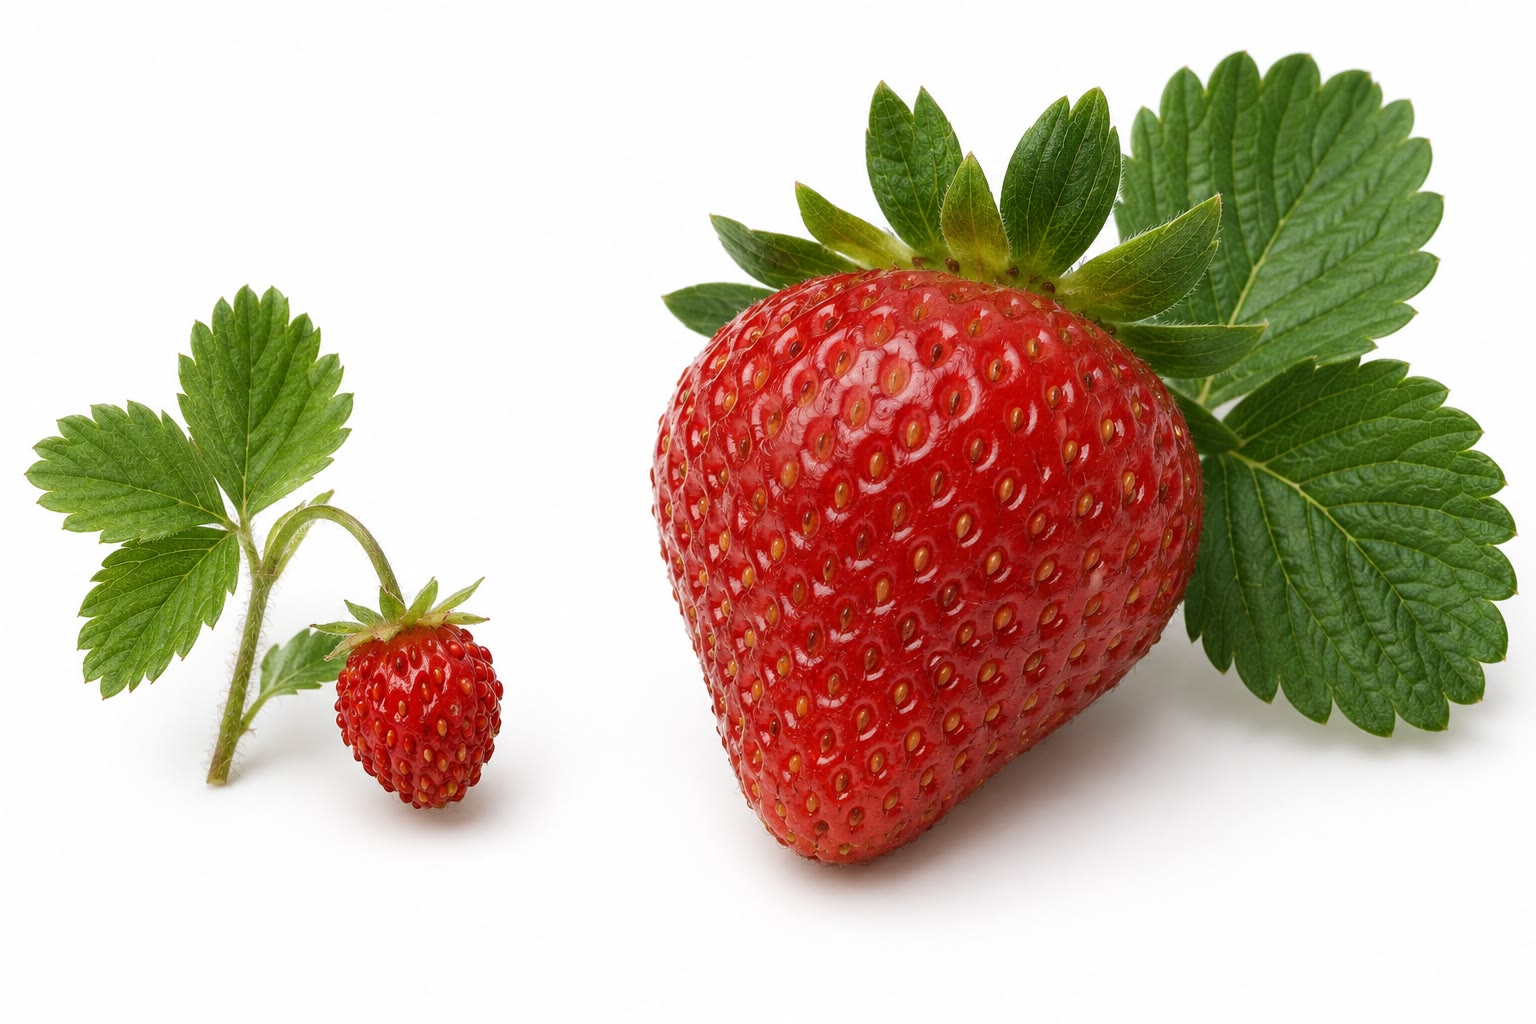
\includegraphics[width=0.55\linewidth]{images/book4/ai/b4-03-polyploid-strawberries.jpg}

{\small Un fraisier sauvage diploïde et le fraisier cultivé octoploïde~:
le \omterm{def:b2:genome-diversification:polyploidy}{polyploïde}, qui a quatre fois plus d'ADN dans chaque cellule, est la
plante la plus grande, aux fruits les plus gros.}
\end{omfigure}

\section{Hasard et vitesse}

\begin{proposition}[La mutation est aléatoire au regard du besoin]\label{prop:b2:genome-diversification:random}
\index{mutation!caractere aleatoire de la@caractère aléatoire de la}
Le \omterm{thm:b2:genome-diversification:luria}{test de fluctuation} et l'étalement sur répliques montrent qu'une
\omterm{def:b2:genome-diversification:mutation}{mutation} utile dans un nouvel environnement apparaît à la même
fréquence, que cet environnement soit présent ou non~: l'environnement
sélectionne parmi les \omterm{def:b2:genome-diversification:mutation}{mutations}, il ne les suscite pas. La \omterm{def:b2:genome-diversification:mutation}{mutation}
n'est pas aléatoire en tous les sens --- les transitions sont plus
nombreuses que les transversions, les dinucléotides CpG mutent dix fois
plus vite que les autres sites (leur cytosine méthylée se désamine en
thymine, que la réparation ne reconnaît pas comme étrangère), certaines
régions sont des points chauds, et le stress peut élever le taux
global --- mais elle est aveugle à ses conséquences. Le \omterm{thm:b2:genome-diversification:rate}{taux de
mutation} lui-même est un caractère héréditaire, que la sélection
ajuste~: trop élevé, chaque génération hérite de changements nuisibles~;
trop faible, la population ne peut pas suivre un monde qui change. Les
souches mutatrices l'emportent brièvement à l'hôpital et perdent à la
longue, et le taux de
$10^{-9}$ par base auquel se fixent la plupart des cellules est un
compromis entre le coût des erreurs et le coût de la relecture.
\end{proposition}

\section{Exercices}

\begin{exercise}[$\star$]\label{exo:b2:genome-diversification:1}
Classer chacune des modifications suivantes du codon GAA (glutamate)~:
GAG~; GTA~; TAA~; insertion d'un C après la première base. Laquelle est
une transition, laquelle une transversion~?
\end{exercise}

\begin{exercise}[$\star$]\label{exo:b2:genome-diversification:2}
Avec $u = \qty{5e-10}{}$ par paire de bases et par réplication et $G =
\qty{4.6e6}{}$, combien de \omterm{def:b2:genome-diversification:mutation}{mutations} nouvelles une division
d'\emph{E.~coli} produit-elle en moyenne~? Combien par génération dans
une culture de
$10^{9}$ cellules~?
\end{exercise}

\begin{exercise}[$\star$]\label{exo:b2:genome-diversification:3}
Nommer les trois voies du \omterm{def:b2:genome-diversification:hgt}{transfert horizontal de gènes} et dire, pour
chacune, ce qu'elle exige (un contact, un virus, de l'ADN libre) et ce
qu'elle transfère typiquement.
\end{exercise}

\begin{exercise}[$\star$]\label{exo:b2:genome-diversification:4}
Distinguer autopolyploïdie et allopolyploïdie, avec un exemple de
chacune, et expliquer pourquoi un hybride diploïde de deux espèces est
en général stérile.
\end{exercise}

\begin{exercise}[$\star\star$]\label{exo:b2:genome-diversification:5}
Une lignée germinale humaine accumule $u = \qty{1.2e-8}{}$ \omterm{def:b2:genome-diversification:mutation}{mutation} par
paire de bases et par génération, sur un génome haploïde de
\qty{3.2e9}{} paires de bases. Combien de \omterm{def:b2:genome-diversification:mutation}{mutations} nouvelles un enfant
porte-t-il~? Si \qty{1.5}{\%} du génome code des protéines et que
\qty{70}{\%} des substitutions codantes changent un acide aminé, combien
de changements d'acides aminés nouveaux l'enfant porte-t-il~?
\end{exercise}

\begin{exercise}[$\star\star$]\label{exo:b2:genome-diversification:6}
Une culture passe de $10^{3}$ à $10^{9}$ cellules~; une \omterm{def:b2:genome-diversification:mutation}{mutation} donnée
survient avec $m = \qty{2e-8}{}$ par division. Calculer le nombre
attendu d'événements mutationnels et de cellules mutantes. Pourquoi la
proportion de cultures sans mutant est-elle ici inutilisable pour
mesurer $m$, et quelle taille de culture la rendrait utilisable~?
\end{exercise}

\begin{exercise}[$\star\star$]\label{exo:b2:genome-diversification:7}
La cytosine se désamine en uracile~; la 5-méthylcytosine se désamine en
thymine. Expliquer pourquoi la première lésion est efficacement réparée
et la seconde non, et en déduire pourquoi les sites CpG (où la cytosine
est méthylée) sont des points chauds de \omterm{def:b2:genome-diversification:mutation}{mutation} et sont plus rares
dans le génome que ne le prédirait le hasard.
\end{exercise}

\begin{exercise}[$\star\star$]\label{exo:b2:genome-diversification:8}
Dans une expérience de conjugaison interrompue, quatre gènes entrent
dans le receveur à 8, 17, 25 et \qty{40}{min}~; le chromosome entier
(\qty{4.6}{Mb}) mettrait \qty{100}{min}. Convertir les temps en
positions en kilobases et calculer les distances entre gènes
consécutifs.
\end{exercise}

\begin{exercise}[$\star\star$]\label{exo:b2:genome-diversification:9}
Schématiser l'appariement et le crossing-over qui transforment deux
chromosomes portant chacun deux gènes d'$\alpha$-globine en tandem en
un chromosome à trois gènes et un chromosome à un gène. Une personne
hérite d'un chromosome à un gène de chacun de ses parents~: combien de
gènes $\alpha$ possède-t-elle, et que peut-on attendre de son
hémoglobine~?
\end{exercise}

\begin{exercise}[$\star\star\star$]\label{exo:b2:genome-diversification:10}
Le blé tendre est AABBDD avec $2n = 42$. Donner le nombre de
chromosomes de ses gamètes, des hybrides stériles à chaque étape de son
origine, et d'un croisement entre blé tendre et amidonnier (AABB).
Expliquer, en termes d'appariement méiotique, pourquoi chaque
doublement a rétabli la fertilité et pourquoi l'hexaploïde ne peut pas
se recroiser avec ses parents.
\end{exercise}

\begin{exercise}[$\star\star\star$]\label{exo:b2:genome-diversification:11}
Dans une population intestinale de $N = 10^{9}$ bactéries, un \omterm{def:b2:unicellular-diversity:prokaryote}{plasmide}
de résistance se propage par conjugaison à une vitesse proportionnelle
aux rencontres entre porteurs $R$ et non-porteurs $N - R$~:
$\mathrm{d}R/\mathrm{d}t =
\gamma R (N - R)$ avec $\gamma N = \qty{0.5}{h^{-1}}$. Résoudre à partir
d'un seul porteur, et calculer le temps au bout duquel la moitié de la
population porte le \omterm{def:b2:unicellular-diversity:prokaryote}{plasmide}. Que se passe-t-il si l'antibiotique est
alors retiré et que le \omterm{def:b2:unicellular-diversity:prokaryote}{plasmide} coûte \qty{5}{\%} de taux de croissance
à son hôte~?
\end{exercise}

\begin{exercise}[$\star\star\star$]\label{exo:b2:genome-diversification:12}
«~La \omterm{def:b2:genome-diversification:mutation}{mutation} est aléatoire~; l'évolution ne l'est pas.~» Discuter, à
l'aide du \omterm{thm:b2:genome-diversification:luria}{test de fluctuation}, de l'étalement sur répliques et du fait
que le \omterm{thm:b2:genome-diversification:rate}{taux de mutation} est lui-même soumis à la sélection.
\end{exercise}

\section{Problème~: un test de fluctuation}

\begin{problem}[{Problème du week-end --- un test de fluctuation est
réalisé et analysé~; le taux de mutation d'une souche en est extrait et
rapporté à son génome et à sa population, la propagation d'un plasmide
de résistance est modélisée et le coût d'un mutateur est évalué,
jusqu'au taux de mutation de la souche par base et au temps que met le
plasmide à envahir la population}]
\label{pb:b2:genome-diversification:1}
Vingt cultures d'\emph{E.~coli} sont lancées chacune à partir de
\num{100} cellules dans \qty{0.2}{mL} et amenées à $N = \qty{2e8}{}$
cellules~; chacune est ensuite étalée sur une boîte avec un
bactériophage, et l'on compte les colonies résistantes~: 0, 0, 0, 1, 0,
0, 3, 0, 0, 1, 0, 0, 0, 0, 107, 0, 2, 0, 0, 5. En parallèle, vingt
échantillons de \qty{0.2}{mL} sont prélevés dans une grande culture de
même densité et étalés de la même manière~: 14, 15, 13, 21, 15, 14,
26, 16, 20, 13, 17, 12, 18, 14, 16, 19, 15, 13, 17, 16. Génome~:
\qty{4.6e6}{} paires de bases, \qty{88}{\%} codantes. La résistance au
phage peut résulter de n'importe lequel de \num{20} changements
distincts d'une seule base dans un gène de récepteur.

\medskip
\noindent\textbf{Partie I --- Le test.}
\begin{enumerate}
  \item Calculer la moyenne et la variance des vingt cultures
        indépendantes.
  \item Calculer la moyenne et la variance des vingt échantillons.
  \item Pour une loi de Poisson, la variance est égale à la moyenne.
        Quelle série suit une loi de Poisson, et que dit la distribution
        de chaque série sur le \emph{moment} où les \omterm{def:b2:genome-diversification:mutation}{mutations} se sont
        produites~?
  \item Expliquer le nombre 107.
  \item Combien de cultures indépendantes ne contiennent aucun mutant~?
        Utiliser $p_0 = e^{-m(N - N_0)}$ pour estimer $m$, le \omterm{thm:b2:genome-diversification:rate}{taux de
        mutation} vers la résistance par division cellulaire.
  \item Calculer le nombre attendu de cellules mutantes par culture à
        partir de $mN\ln(N/N_0)$ et le comparer à la moyenne observée.
  \item Pourquoi les échantillons de la culture unique auraient-ils été
        inutilisables pour estimer $m$ par la méthode de $p_0$~?
\end{enumerate}

\medskip
\noindent\textbf{Partie II --- Du gène au génome.}
\begin{enumerate}[resume]
  \item En déduire le \omterm{thm:b2:genome-diversification:rate}{taux de mutation} $u$ par paire de bases et par
        réplication, à partir de $m$ et du nombre de changements
        conférant la résistance.
  \item Calculer le nombre moyen de \omterm{def:b2:genome-diversification:mutation}{mutations} nouvelles par génome et
        par réplication, $U$.
  \item Une culture d'un litre à $10^{9}$ cellules par millilitre double
        une fois. Combien de \omterm{def:b2:genome-diversification:mutation}{mutations} nouvelles apparaissent dans la
        population~?
  \item Combien de changements distincts d'une seule base sont possibles
        dans ce génome~? En moyenne, combien de fois chacun apparaît-il
        au cours de ce seul doublement~?
  \item Expliquer pourquoi, dans une telle population, la résistance à
        tout antibiotique qu'une seule \omterm{def:b2:genome-diversification:mutation}{mutation} peut mettre en échec est
        pratiquement assurée d'être présente.
  \item Expliquer pourquoi l'association de deux antibiotiques exigeant
        deux \omterm{def:b2:genome-diversification:mutation}{mutations} indépendantes change la situation, chiffre à
        l'appui.
\end{enumerate}

\medskip
\noindent\textbf{Partie III --- Un \omterm{def:b2:unicellular-diversity:prokaryote}{plasmide} se propage.}
Dans un intestin contenant $N = 10^{9}$ cellules, une cellule acquiert
un \omterm{def:b2:unicellular-diversity:prokaryote}{plasmide} conjugatif de résistance. Les porteurs $R$ le transmettent
par contact~:
$\mathrm{d}R/\mathrm{d}t = \gamma R(N - R)$, avec $\gamma N =
\qty{0.5}{h^{-1}}$.
\begin{enumerate}[resume]
  \item Montrer que $R(t) = N/\bigl(1 + (N - 1)e^{-\gamma N t}\bigr)$
        est solution de l'équation avec $R(0) = 1$.
  \item Calculer le temps au bout duquel la moitié des cellules portent
        le \omterm{def:b2:unicellular-diversity:prokaryote}{plasmide}.
  \item Calculer le temps au bout duquel \qty{99}{\%} le portent.
  \item Combien d'événements de conjugaison ont lieu par heure au moment
        où la moitié des cellules sont porteuses~?
  \item Comparer avec le temps qu'il faut à un \emph{mutant} résistant
        pour atteindre la moitié de la population en croissant
        \qty{10}{\%} plus vite que les autres sous antibiotique (\omterm{def:b2:unicellular-diversity:division}{temps de
        génération} \qty{1}{h} pour les cellules sensibles)~: combien de
        temps faut-il à partir d'une seule cellule~?
  \item Conclure sur la raison pour laquelle la résistance se propage
        surtout par transfert plutôt que par descendance.
\end{enumerate}

\medskip
\noindent\textbf{Partie IV --- Un mutateur.}
Une souche dépourvue de réparation des mésappariements mute \num{100}
fois plus vite. On suppose que \qty{30}{\%} des \omterm{def:b2:genome-diversification:mutation}{mutations} dans une
séquence codante sont nuisibles.
\begin{enumerate}[resume]
  \item Calculer son $U$ et le nombre moyen de \omterm{def:b2:genome-diversification:mutation}{mutations} nuisibles par
        cellule et par génération.
  \item Au bout de \num{200} générations, quelle fraction des
        descendants d'une lignée ne porte aucune \omterm{def:b2:genome-diversification:mutation}{mutation} nuisible
        (loi de Poisson)~?
  \item Calculer la même fraction pour le type sauvage.
  \item Dans le \omterm{thm:b2:genome-diversification:luria}{test de fluctuation} ci-dessus, quel nombre moyen le
        mutateur aurait-il donné, et quelle proportion de cultures sans
        mutant~?
  \item Expliquer en deux phrases pourquoi on trouve des mutateurs parmi
        les isolats hospitaliers et pourquoi ils sont rares dans la
        nature.
  \item Énoncer le résultat~: $m$, $u$, $U$ pour la souche, et les temps
        au bout desquels le \omterm{def:b2:unicellular-diversity:prokaryote}{plasmide} atteint la moitié et \qty{99}{\%}
        de l'intestin.
\end{enumerate}
\end{problem}
